\chapter{The Gaussian Process}\label{chap:theory}

\section{The Multivariate Gaussian Distribution}
The Gaussian Distribution is one one the most used distributions in statistics \cite{murphy} and generalizes well into the multivariate case. The pdf for the $D$ dimensional multivariate Gaussian is given by \cref{eq:multivariate_gaussian} \cite{murphy}.
\begin{equation}\label{eq:multivariate_gaussian}
    \mathcal{N}(\boldsymbol{x} \; | \; \boldsymbol{\mu}, \boldsymbol{\Sigma}) \triangleq \frac{1}{(2 \pi)^{D/2} |\boldsymbol{\Sigma} | ^{1/2}} \exp \bigg[- \frac{1}{2} (\boldsymbol{x} - \boldsymbol{\mu})^\intercal \boldsymbol{\Sigma}^{-1}(\boldsymbol{x} - \boldsymbol{\mu})\bigg]
\end{equation}
\subsection{Marginalization and conditioning}
Consider a joint multivariate Gaussian distribution for two (possibly vector-valued) variables $\boldsymbol{x}$ and $\boldsymbol{y}$.
\begin{equation}
    p(\boldsymbol{x}, \boldsymbol{y}) = N\bigg(\begin{bmatrix}
        \boldsymbol{x} \\ \boldsymbol{y}
    \end{bmatrix} \; \bigg| \; \begin{bmatrix}
        \boldsymbol{\mu}_x \\ \boldsymbol{\mu}_y
    \end{bmatrix}, \begin{bmatrix}
        \boldsymbol{\Sigma_{xx}} &
        \boldsymbol{\Sigma_{xy}} \\
        \boldsymbol{\Sigma_{yx}} &
        \boldsymbol{\Sigma_{yy}}
    \end{bmatrix}\bigg)
\end{equation}
The marginals are then given by \cref{eq:multivariate_gaussian_marginal} and can simply be calculated by picking the corresponding values from $\boldsymbol{\mu}$ $\boldsymbol{\Sigma}$, i.e. no calculations needed. 
\begin{align}\label{eq:multivariate_gaussian_marginal}
    \begin{split}
    p(\boldsymbol{x}) &= \mathcal{N}(\boldsymbol{x} \; | \; \boldsymbol{\mu}_x, \boldsymbol{\Sigma}_{xx})\\
    p(\boldsymbol{y}) &= \mathcal{N}(\boldsymbol{y} \; | \; \boldsymbol{\mu}_y, \boldsymbol{\Sigma}_{yy})
    \end{split}
    \end{align}
 The posterior conditional is given by \cref{eq:multivariate_gaussian_conditional}. These equations will be used extensively throughout this thesis.
 \begin{tcolorbox}[title={Posterior Conditional Distribution}]
 \begin{subequations}\label{eq:multivariate_gaussian_conditional}
 \begin{align}
    p(\boldsymbol{x} | \boldsymbol{y}) &= \mathcal{N}(\boldsymbol{x} \; | \; \boldsymbol{\mu}_{x|y}, \boldsymbol{\Sigma}_{x|y})\\
    \boldsymbol{\mu}_{x|y} &= \boldsymbol{\mu}_x + \boldsymbol{\Sigma}_{xy}\boldsymbol{\Sigma}_{yy}^{-1}(\boldsymbol{y} - \boldsymbol{\mu}_y)\\
    \boldsymbol{\Sigma}_{x|y} &= \boldsymbol{\Sigma}_{xx} -\boldsymbol{\Sigma}_{xy}\boldsymbol{\Sigma}_{yy}^{-1}\boldsymbol{\Sigma}_{yx}
 \end{align}
 \end{subequations}
 \end{tcolorbox}


\section{Introduction to Gaussian Processes}

This introduction is heavily inspired by \cite{rasmussen} where more details can be found for those interested. 

A \acrfull{gp} can formally be defined as Definition \ref{def:gp}.

\newtheorem{gp_def}{Definition}
\begin{gp_def}\label{def:gp}
A Gaussian Process is a collection of random variables, any finite number of which has a joint Gaussian Distribution.
\end{gp_def}

In this thesis we will use a more specific definition in order to interpret \acrshort{gp}'s as a statistical distribution over functions. A \acrshort{gp} for a random function $f \triangleq f(\boldsymbol{x})$ is fully specified by its mean function $m(\boldsymbol{x})$ and covariance function $k(\boldsymbol{x}, \boldsymbol{x}')$.

\begin{equation}\label{eq:gp}
    f \sim GP(\;m(\boldsymbol{x}), \; k(\boldsymbol{x}, \boldsymbol{x}')\;)
\end{equation}

This interpretation of a \acrshort{gp} might seem a bit odd at first. The key observation is that the marginal distribution $p(\boldsymbol{x})$ of a multivariate Gaussian distribution $p(\boldsymbol{x}, \boldsymbol{y})$ is another Gaussian distribution that is completetly independent of $\boldsymbol{y}$, as expressed in \cref{eq:multivariate_gaussian_marginal}. Any variables not of interest can therefore easily be marginalized away, leaving only the subset of variables we care about.

Any \acrshort{gp} by Definition \ref{def:gp} can therefore be thought of as the finite marginal distribution of an infinite Gaussian Distribution, jointly describing the values of $f$ at all possible inputs $\boldsymbol{x}$. In the end, a \acrshort{gp} is nothing more than a joint Gaussian Distribution with a fancy interpretation.

\subsection{A quick note on vector notation}
We use two different notations for vector values in order to differentiate between two common cases:
\begin{description}
\item[Bold letters] are used to indicate a single, multivariate value. $f(\boldsymbol{x})$ is the scalar function $f$ evaluated at the multivariate input $\boldsymbol{x}$. In practice, this implies the input is $\boldsymbol{x} \in \mathcal{R}^{1 x M}$ with $M\geq 2$ columns.
\item[Capital letters] such as X, are used to indicate multiple (potentially multivariate) samples. $f(X)$ is the scalar function $f$ evaluated at each row in $X$. In practice this implies that the input $X \in \mathcal{R}^{N x M}$ with $N \geq 2$ rows (samples) and $M \geq 1$ columns (dimensions).
\end{description}

\subsection{Introduction to kernels}
The covariance function $k(\boldsymbol{x}, \boldsymbol{x}')$ determines the similarity between two different points $\boldsymbol{x}$ and $\boldsymbol{x}'$. These covariance functions will in this theis be referred to as a \textit{kernel}, which maps the input space to a \textit{feature-space} \cite{rasmussen}. The key idea behind kernels is that the kernels may in many cases be simpler to compute than the input vectors themselves if the input-space is complex. The output of the kernel is a value describing the similarity (i.e. covariance) between the two inputs. Different types of kernels will be discussed in greater detail in \cref{sec:kernels}.

The kernel must be positive definite in order to produce a valid covariance matrix, which requires that

\begin{equation}
    k(\boldsymbol{x}, \boldsymbol{x}') = k(\boldsymbol{x}', \boldsymbol{x})
\end{equation}

The resulting covariance matrix $K(X, X)$ is the result of calling $k(\cdot, \cdot)$ on all pairs on inputs, i.e.
\begin{equation}
    K(X, X)_{ij} = k(\boldsymbol{x}_i, \boldsymbol{x}_j) \quad \forall i, j
\end{equation}

\subsection{Conditioning}
So far we have only specified the prior distribution for $f$. As a \acrshort{gp} is by definition a multivariate Gaussian Distribution, the posterior conditional in \cref{eq:multivariate_gaussian_conditional} can be used to condition $f$ on observed values. 
As an example, we use a simple \acrshort{gp} for $f$ with mean $m$ and kernel $k$.

Let $\boldsymbol{f}_* \triangleq f(X_*)$ denote the function evaluated at test points $X_*$. Before any observations are made we can only rely on prior information as shown in \cref{fig:gp_prior}. From a Bayesian perspective, we want to update our prior beliefs after observing $\boldsymbol{y} = f(X) + \epsilon$ at multiple inputs $X$ to get the posterior belief $\boldsymbol{f}_* \; | X, \boldsymbol{y}, X_*$.

The joint distribution of $\boldsymbol{y}$ and $\boldsymbol{f}_*$ is given by 

\begin{equation}
    p(\boldsymbol{y}, \boldsymbol{f}_*) = \mathcal{N}\bigg(\begin{bmatrix}
        \boldsymbol{y} \\ \boldsymbol{f}_*
    \end{bmatrix} \; \bigg| \begin{bmatrix}
        m(X) \\ m(X_*)
    \end{bmatrix},  \begin{bmatrix}
        K(X, X) & K(X, X_*) \\ K(X_*, X) & K(X_*, X_*)
    \end{bmatrix}\bigg)
\end{equation}

The posterior distribution $\boldsymbol{f}_* | \boldsymbol{y}$ can easily be computed using the closed form solution in \cref{eq:multivariate_gaussian_conditional}.
\begin{subequations}\label{eq:gp_conditional}
\begin{align}
    p(\boldsymbol{f}_* | \boldsymbol{y}) &= \mathcal{N}(f \; | \; \boldsymbol{\mu}_{\boldsymbol{f}_*|\boldsymbol{y}}, \boldsymbol{\Sigma}_{\boldsymbol{f}_*|\boldsymbol{y}})\\
    \bar{\boldsymbol{f}}_* = \boldsymbol{\mu}_{\boldsymbol{f}_* | \boldsymbol{y}} &= m(X_*) + K(X_*, X) \; K(X, X)^{-1} \; (\boldsymbol{y} - m(X))\label{eq:gp_conditional_mean}\\
    \mathbb{V}[\boldsymbol{f}_*] = \boldsymbol{\Sigma}_{\boldsymbol{f}_* | \boldsymbol{y}} &= K(X_*, X_*) - K(X_*, X)  K(X, X)^{-1} \; K(X, X_*)\label{eq:gp_conditional_var}
\end{align}
\end{subequations}

As the notation quickly gets messy for the general case, we also introduce a shorthand notation for evaluating $f(\boldsymbol{x}_*)$, which is what we most often want. As used by \cite{rasmussen}, we introduce $\boldsymbol{k}_* = K(X, \boldsymbol{x}_*)$ as a vector of covariances calculated between the test point and each of the training samples, as well as $K=K(X, X)$. Using this shorthand notation for a single test case, \cref{eq:gp_conditional} boils down to \cref{eq:gp_conditional_simple}.

\begin{subequations}\label{eq:gp_conditional_simple}
\begin{align}
    \bar{f}_* &= m(\boldsymbol{x}_*) + \boldsymbol{k}_*^\intercal ( K + \sigma I)^{-1} (\boldsymbol{y} - m(X))\\
    \mathbb{V}[f_*] &= k(\boldsymbol{x}_*, \boldsymbol{x}_*) - \boldsymbol{k}_*^\intercal K^{-1} \; \boldsymbol{k}_*\label{eq:gp_conditional_var}
\end{align}
\end{subequations}

In practice, computing the inverse $K(X, X)$ quickly becomes expensive for increasing number of samples. To avoid numerical instability, the \textit{Cholesky Decomposition} is usually preferred. The Cholesky Decomposition forms a new lower-triangular matrix $L$ such that $K = L L^\intercal$, and can be seen as the matrix equivalent of the square root. \cref{eq:gp_conditional} can then be computed using $L$. A small diagonal entry is also usually added to the kernel matrix, i.e. $K' = K + \sigma I$ to model noisy observations. This modification also improves the numerical stability, so a small value is recommended even if the observations are noise free \cite{scikit-learn}.
\begin{subequations}
\begin{align}
    \begin{split}
    \bar{\boldsymbol{f}}_* &= m(X_*) + K(X_*, X) \; (L L^\intercal)^{-1} \; (\boldsymbol{y} - m(X))\\ &= m(X_*) + K(X_*, X) \; \underbrace{\big[(L^\intercal)^{-1} (L)^{-1}  \; (\boldsymbol{y} - m(X))\big]}_{\boldsymbol{\alpha}}
    \end{split}\\
    \begin{split}
    \mathbb{V}[\boldsymbol{f}_*] &= K(X_*, X_*) - K(X_*, X) \; (L L^\intercal)^{-1} \; K(X, X_*)\\
    &= K(X_*, X_*) - K(X_*, X) \; (L^\intercal)^{-1} (L)^{-1} \; K(X, X_*)\\
    &= K(X_*, X_*) - \underbrace{\big[(L)^{-1} \; K(X, X_*)\big]^\intercal}_{\boldsymbol{v^\intercal}} \; \underbrace{\big[(L)^{-1} \; K(X, X_*)\big]}_{\boldsymbol{v}}
    \end{split}
\end{align}
\end{subequations}

This boils down to \cref{alg:gp_prediction} as proposed by \cite{rasmussen}. A simple \acrshort{gp} before and after conditioning is shown in \cref{fig:gp_simple}
\begin{algorithm}[h]
\begin{algorithmic}[1]
    
\Procedure{GP-PREDICT}{$X_*$, $\boldsymbol{y}$, $k$, $X$}
    \State $L = cholesky\big(K(X, X) + \sigma I\big)$
    \State $\boldsymbol{\alpha} = L^\intercal \backslash (L \backslash \boldsymbol{y})$
    \State $\boldsymbol{v} = L \backslash K(X, X_*)$
    \State $\bar{\boldsymbol{f}}_* = m(X_*) + K(X_*, X) \boldsymbol{\alpha}$
    \State $\mathbb{V}[\boldsymbol{f}_*] = K(X_*, X_*) - \boldsymbol{v}^\intercal \boldsymbol{v}$
\EndProcedure
\end{algorithmic}
\caption{Gaussian Process Prediction}
\label{alg:gp_prediction}
\end{algorithm}

\begin{figure}[h]
    \centering
    \begin{subfigure}{0.49\textwidth}
        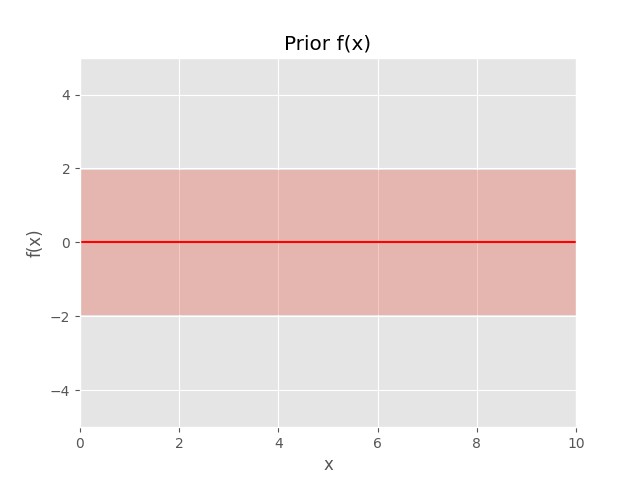
\includegraphics[width=\textwidth]{figures/introduction-gp/prior.png}
        \caption{Prior}
        \label{fig:gp_prior}
    \end{subfigure}
    \begin{subfigure}{0.49\textwidth}
        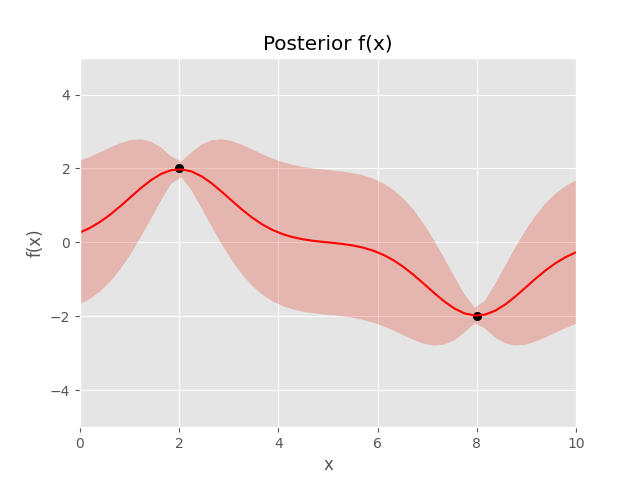
\includegraphics[width=\textwidth]{figures/introduction-gp/posterior.png}
        \caption{Posterior after observing the function at two different inputs (black dots).}
        \label{fig:gp_posterior}
    \end{subfigure}
    \caption{Simple Gaussian Process example with zero-mean and \acrshort{rbf} kernel with unit variance. The red line is the mean, while the red area is the $95\%$ confidence interval.}
    \label{fig:gp_simple}
\end{figure}

\section{Vector-valued Gaussian Process}
\acrshort{gp}s can easily be extended for vector-valued functions by simply considering the joint distribution of each function component as in \cref{eq:gp_vector}. In this thesis we will assume independent components, i.e. $k_{xy}=k_{yx}=0$
\begin{equation}\label{eq:gp_vector}
     \vec{f}(\boldsymbol{x}) = \begin{bmatrix} f_x (\boldsymbol{x})\\ f_y (\boldsymbol{x})\end{bmatrix} \sim \text{GP} \big(\begin{bmatrix} m_x(\boldsymbol{x})\\m_y(\boldsymbol{x})\end{bmatrix}, \ \begin{bmatrix}
    k_{xx}(\boldsymbol{x}, \boldsymbol{x}') & k_{xy}(\boldsymbol{x}, \boldsymbol{x}') \\ k_{xy}(\boldsymbol{x}, \boldsymbol{x}')^\intercal & k_{yy}(\boldsymbol{x}, \boldsymbol{x}')
    \end{bmatrix}\big) 
\end{equation}

\section{Model Selection}
\section{Kernels}\label{sec:kernels}
\subsection{Radial Basis Function}\label{sec:kernels_rbf}

\section{Extended Kalman Filter}
\section{Particle Filter}
\section{Multivariate Gaussian Process}
\section{Computational Complexity}
\section{Approximate methods}
\subsection{Variational Inference}
\subsection{Markov Chain Monte Carlo}
